\documentclass{beamer}
\mode<presentation> {
\usetheme{Madrid}
}

\usepackage{amsmath,amsthm,amssymb,amsfonts}
\usepackage{enumerate}
\usepackage{graphicx} % Allows including images
\usepackage{color}

\usepackage{booktabs} % Allows the use of \toprule, \midrule and \bottomrule in tables
\usepackage{caption}
\usepackage{algorithm} 
\usepackage{algpseudocode}
%\usepackage[style=verbose, backend=bibtex,maxcitenames=4]{biblatex}
%\addbibresource{references.bib}
%{\footnotesize
%\bibliography{references}}

%%change footnotecite
%\renewcommand*{\thefootnote}{[\arabic{footnote}]}
%\makeatletter
%% Remove superscript for footnotemark
%\def\@makefnmark{\hbox{{\normalfont\@thefnmark}}}
%% Allow space to precede the footnote
%\usepackage{etoolbox}
%\patchcmd{\blx@mkbibfootnote}{\unspace}{}{}
%\makeatother
\usepackage{bbm}
%\usepackage{natbib} 
\setbeamertemplate{bibliography item}{}
\setbeamertemplate{theorems}[numbered]
\newtheorem{thm}{Theorem}
\newtheorem{lem}[thm]{Lemma}
\newtheorem{cor}{Corollary}
\newtheorem*{defi*}{Definition}
\newcommand{\G}{c}
\providecommand{\mb}[1]{\boldsymbol{#1}}
\providecommand{\sct}[1]{{\normalfont\textsc{#1}}}
\providecommand{\mt}[1]{\widetilde{#1}}
\newcommand{\Real}{\mathbb{R}}
\newcommand{\Mgc}{\textbf{\sct{Mgc}}}
\newcommand{\mbx}{\ensuremath{\mb{x}}}
\newcommand{\mby}{\ensuremath{\mb{y}}}

\title[JSM2016]{Dependence Discovery via Multiscale Generalized Correlation} 

\author{Cencheng Shen} % Your name
\institute[] % Your institution as it will appear on the bottom of every slide, may be shorthand to save space
{
\textit{Joint Work with Joshua T. Vogelstein \& Mauro Maggioni \& Carey E. Priebe} \\
%\medskip
%\medskip
%\medskip
%Department of Statistics \\
%Temple University \\  % Your institution for the title page
%https://github.com/jovo/MGC
}
\date{August, 2016} % Date, can be changed to a custom date

\AtBeginSection{\frame{\sectionpage}}

\begin{document}
\bibliographystyle{ieeetr}
\begin{frame}
\titlepage % Print the title page as the first slide
\end{frame}
%1. Intro; 2. it is linear regression and classification; 3. its origin, and why we start investigation; 4. explain title

\begin{frame}
\frametitle{Overview} % Table of contents slide, comment this block out to remove it
\tableofcontents % Throughout your presentation, if you choose to use \section{} and \subsection{} commands, these will automatically be printed on this slide as an overview of your presentation
\end{frame}

\section{Motivations}
\begin{frame}{Motivations}
Given a set of paired observations, testing independence is one of the most important and fundamental tasks in statistics and data science.

\pause
\medskip
Prior to embarking on a predictive machine-learning investigation, one might first check whether any dependence is detectable.

\pause
\medskip
There are many real-data applications that existing methods fall short of in detecting associations.

\pause
\medskip
Modern data sets may be \textbf{high-dimensional, nonlinear, noisy, of small sample size, from disparate spaces}, etc.
\end{frame}

\begin{frame}
We desire a test that

\pause
\medskip
\begin{itemize}[<+->]
\item is consistent as the sample size increases to infinity for most dependencies.
\item has a good finite-sample testing power, for data of low or high dimensionality, linear or non-linearity, small sample size, with noise, etc.
\item does not inflate the false positive rate in the absence of dependency.
\item is easy and efficient to work with for complicated data.
\item provides insights into the dependency structure.
\end{itemize}
\pause
\medskip

To that end, we propose \textbf{multiscale generalized correlation} in [\textit{Shen et al.(2016)}]\cite{ShenEtAl2016}.

\pause
\medskip
\Mgc~combines distance correlation and nearest-neighbor, and is able to satisfy all of the above.
% for testing independence, which combines distance correlation and nearest-neighbor into the same framework.
\end{frame}

\section{Results}
\begin{frame}{Generalized Correlation Coefficient}
Start with $n$ pairs of observations $(\mb{x}_i,\mb{y}_i)$ for $i=1,\ldots,n$, where $\mb{x}$'s and $\mb{y}$'s both might be vectors of arbitrary dimensions, shapes, networks, etc.  

\pause
\medskip
Define a comparison function for each, i.e., $a_{ij}=\delta_x(\mb{x}_i,\mb{x}_j)$, $b_{ij}=\delta_y(\mb{y}_i,\mb{y}_j)$. 
 
\pause
\medskip
Then $A=\{a_{ij}\}$ and $B=\{b_{ij}\}$ are the $n \times n$ interpoint comparison matrices for $X=\{\mb{x}_{i}\}$ and $Y=\{\mb{y}_{i}\}$, respectively. Assuming $\{a_{ij}\}$ and $\{b_{ij}\}$ have zero mean, a generalized correlation coefficient can then be written:

\pause
\begin{equation}
\label{generalCoef}
\G= \tfrac{1}{z} {\textstyle \sum_{i,j=1}^n a_{ij} b_{ij}},
\end{equation}
where $z$ is proportional to standard deviations of $A$ and $B$, that is $z=n^2\sigma_a \sigma_b$.
\end{frame}

\begin{frame}{Examples}
A few examples of $\G$:
\begin{itemize}[<+->]
\item The Pearson's product-moment correlation coefficient by taking $a_{ij}=x_i$ and $b_{ij}=y_i$.
\item The Spearman and Kendall's rank correlations by setting $a_{ij}$ to be $rank(x_i)-rank(x_j)$ and $sign(x_i-x_j)$ respectively.
\item The Mantel coefficient [\textit{Mantel (1967)}]\cite{Mantel1967} by using $a_{ij}=|x_i-x_j|_{2}$ (i.e. Euclidean distance).
\item The distance correlation [\textit{Szekely et al.(2007)}]\cite{SzekelyRizzoBakirov2007} by using the doubly-centered distance entries for $a_{ij}$ and $b_{ij}$.
\item The modified distance correlation [\textit{Szekely and Rizzo (2013)}] \cite{SzekelyRizzo2013a} by slightly tweaking $a_{ij}/b_{ij}$ of dcorr.
\end{itemize}
\end{frame}

\begin{frame}{Rank-truncated pairwise comparisons}
Multiscale Generalized Correlation (\Mgc) combines generalized correlation coefficients with locality, i.e., calculate the correlation between two sparse matrices based on nearest-neighbor.

\pause
\medskip
Let $R(a_{ij})$  be the ``rank'' of $\mb{x}_i$ relative to $\mb{x}_j$, and similarly $R(b_{ij})$ for the \mby's. For any neighborhood size $k$ around each $\mb{x}_i$~and any neighborhood size $l$ around each $\mb{y}_i$, we define the rank-truncated pairwise comparisons:

\pause
\begin{equation}
\label{localCoef2}
    \mt{a}_{ij}^k=
    \begin{cases}
      a_{ij}, & \text{if } R(a_{ij}) \leq k, \\
       % -\bar{a}^{k}, & \text{otherwise};      
      0, & \text{otherwise};
    \end{cases} \qquad \qquad
    \mt{b}_{ij}^l=
    \begin{cases}
      b_{ij}, & \text{if } R(b_{ji}) \leq l, \\
       % -\bar{b}^{l}, & \text{otherwise};
      0, & \text{otherwise}.
    \end{cases}
\end{equation}

\pause
Then let $a^k_{ij}=\mt{a}^k_{ij} - \bar{a}^k$, where $\bar{a}^k$ is the mean, and $b^k_{ij}$ similarly.
\end{frame}

\begin{frame}{Local Correlations}
We can therefore define a \emph{local} variant of any global generalized correlation coefficient by  excluding large distances: 

\pause
\medskip
\begin{equation}
\label{localCoef}
\G^{kl}=\dfrac{1}{z_{kl}} {\textstyle \sum_{i,j=1}^n a_{ij}^k b_{ij}^l},
\end{equation}

\pause
\medskip
where $z_{kl}=n^2 \sigma_a^k \sigma_b^l$ with $\sigma_a^k$ and $\sigma_b^{l}$ being the standard deviations for the truncated pairwise comparisons. 

\pause
\medskip
There are a maximum of $n^2$ different local correlations, and they are always symmetric, i.e. $\G^{kl}(X,Y)=\G^{lk}(Y,X)$, no matter $A$ and $B$ are symmetric or not.
\end{frame}

\subsection{Multiscale Generalized Correlation}
\begin{frame}{MGC}
In $\{\G_{kl}\}$, the optimal local correlation (with respect to the independence testing power) exists, is distribution dependent, and may not be unique.

\pause
\medskip
The optimal local correlation coefficient is dubbed as the multiscale graph correlation $\G^{*}$.

\pause
\medskip
Each local correlation requires $O(n^2)$ to compute. However, once $A$ and $B$ are sorted, \textbf{all local correlations can be simultaneously calculated in $O(n^2)$ as well!!!}
\end{frame}

\begin{frame}{The Testing Framework}
The formal testing scenario is as follows: assume that $\mb{x}_i, i=1,\ldots,n$ are identically independently distributed (i.i.d.) as $\mb{x} \sim f_{x}$; similarly each $\mb{y}_{i}$ are i.i.d. as $\mb{y} \sim f_{y}$. 

\pause
\medskip
The null and the alternative hypothesis for testing independence are
\begin{align*}
& H_{0}: f_{xy}=f_{x}f_{y},\\
& H_{A}: f_{xy} \neq f_{x}f_{y},
\end{align*}
where $f_{xy}$ denotes the joint distribution of $(\mb{x},\mb{y})$. 

\pause
\medskip
To test on a pair of sample data, we use the p-value of a permutation test.% and reject the null when the p-value is sufficiently small.

\pause
\medskip
A test is universally consistent if its power converges to $1$ as $n \rightarrow \infty$ whenever $f_{xy} \neq f_x f_y$.

\pause
\medskip
But we all want a test with high power in finite-sample rather than asymptotically!
%The power of a test is defined as the probability that it correctly rejects the null when the null is indeed false, and has power equal to the type $1$ error level when the null is true. And a test is universally consistent if its power converges to $1$ as $n \rightarrow \infty$ whenever $f_{xy} \neq f_x f_y$.
\end{frame}

\subsection{Theoretical Advantages}
\begin{frame}{Theorems of MGC}
\begin{thm}
\Mgc~is theoretically consistent against all dependent alternatives for which its global counterpart is. 
\end{thm}

\pause
\medskip
\begin{thm}
If $\mb{x}$ is linearly dependent on $\mb{y}$, then the optimal scale for \Mgc~is always the global scale.
\end{thm}

\pause
\medskip
\begin{thm}
There exists $f_{xy}$ and $n$ such that \Mgc~is better than its global counterpart in testing power.
\end{thm}
\end{frame}

\begin{frame}{Illustration of Utilizing locality}
\begin{figure}[htbp]
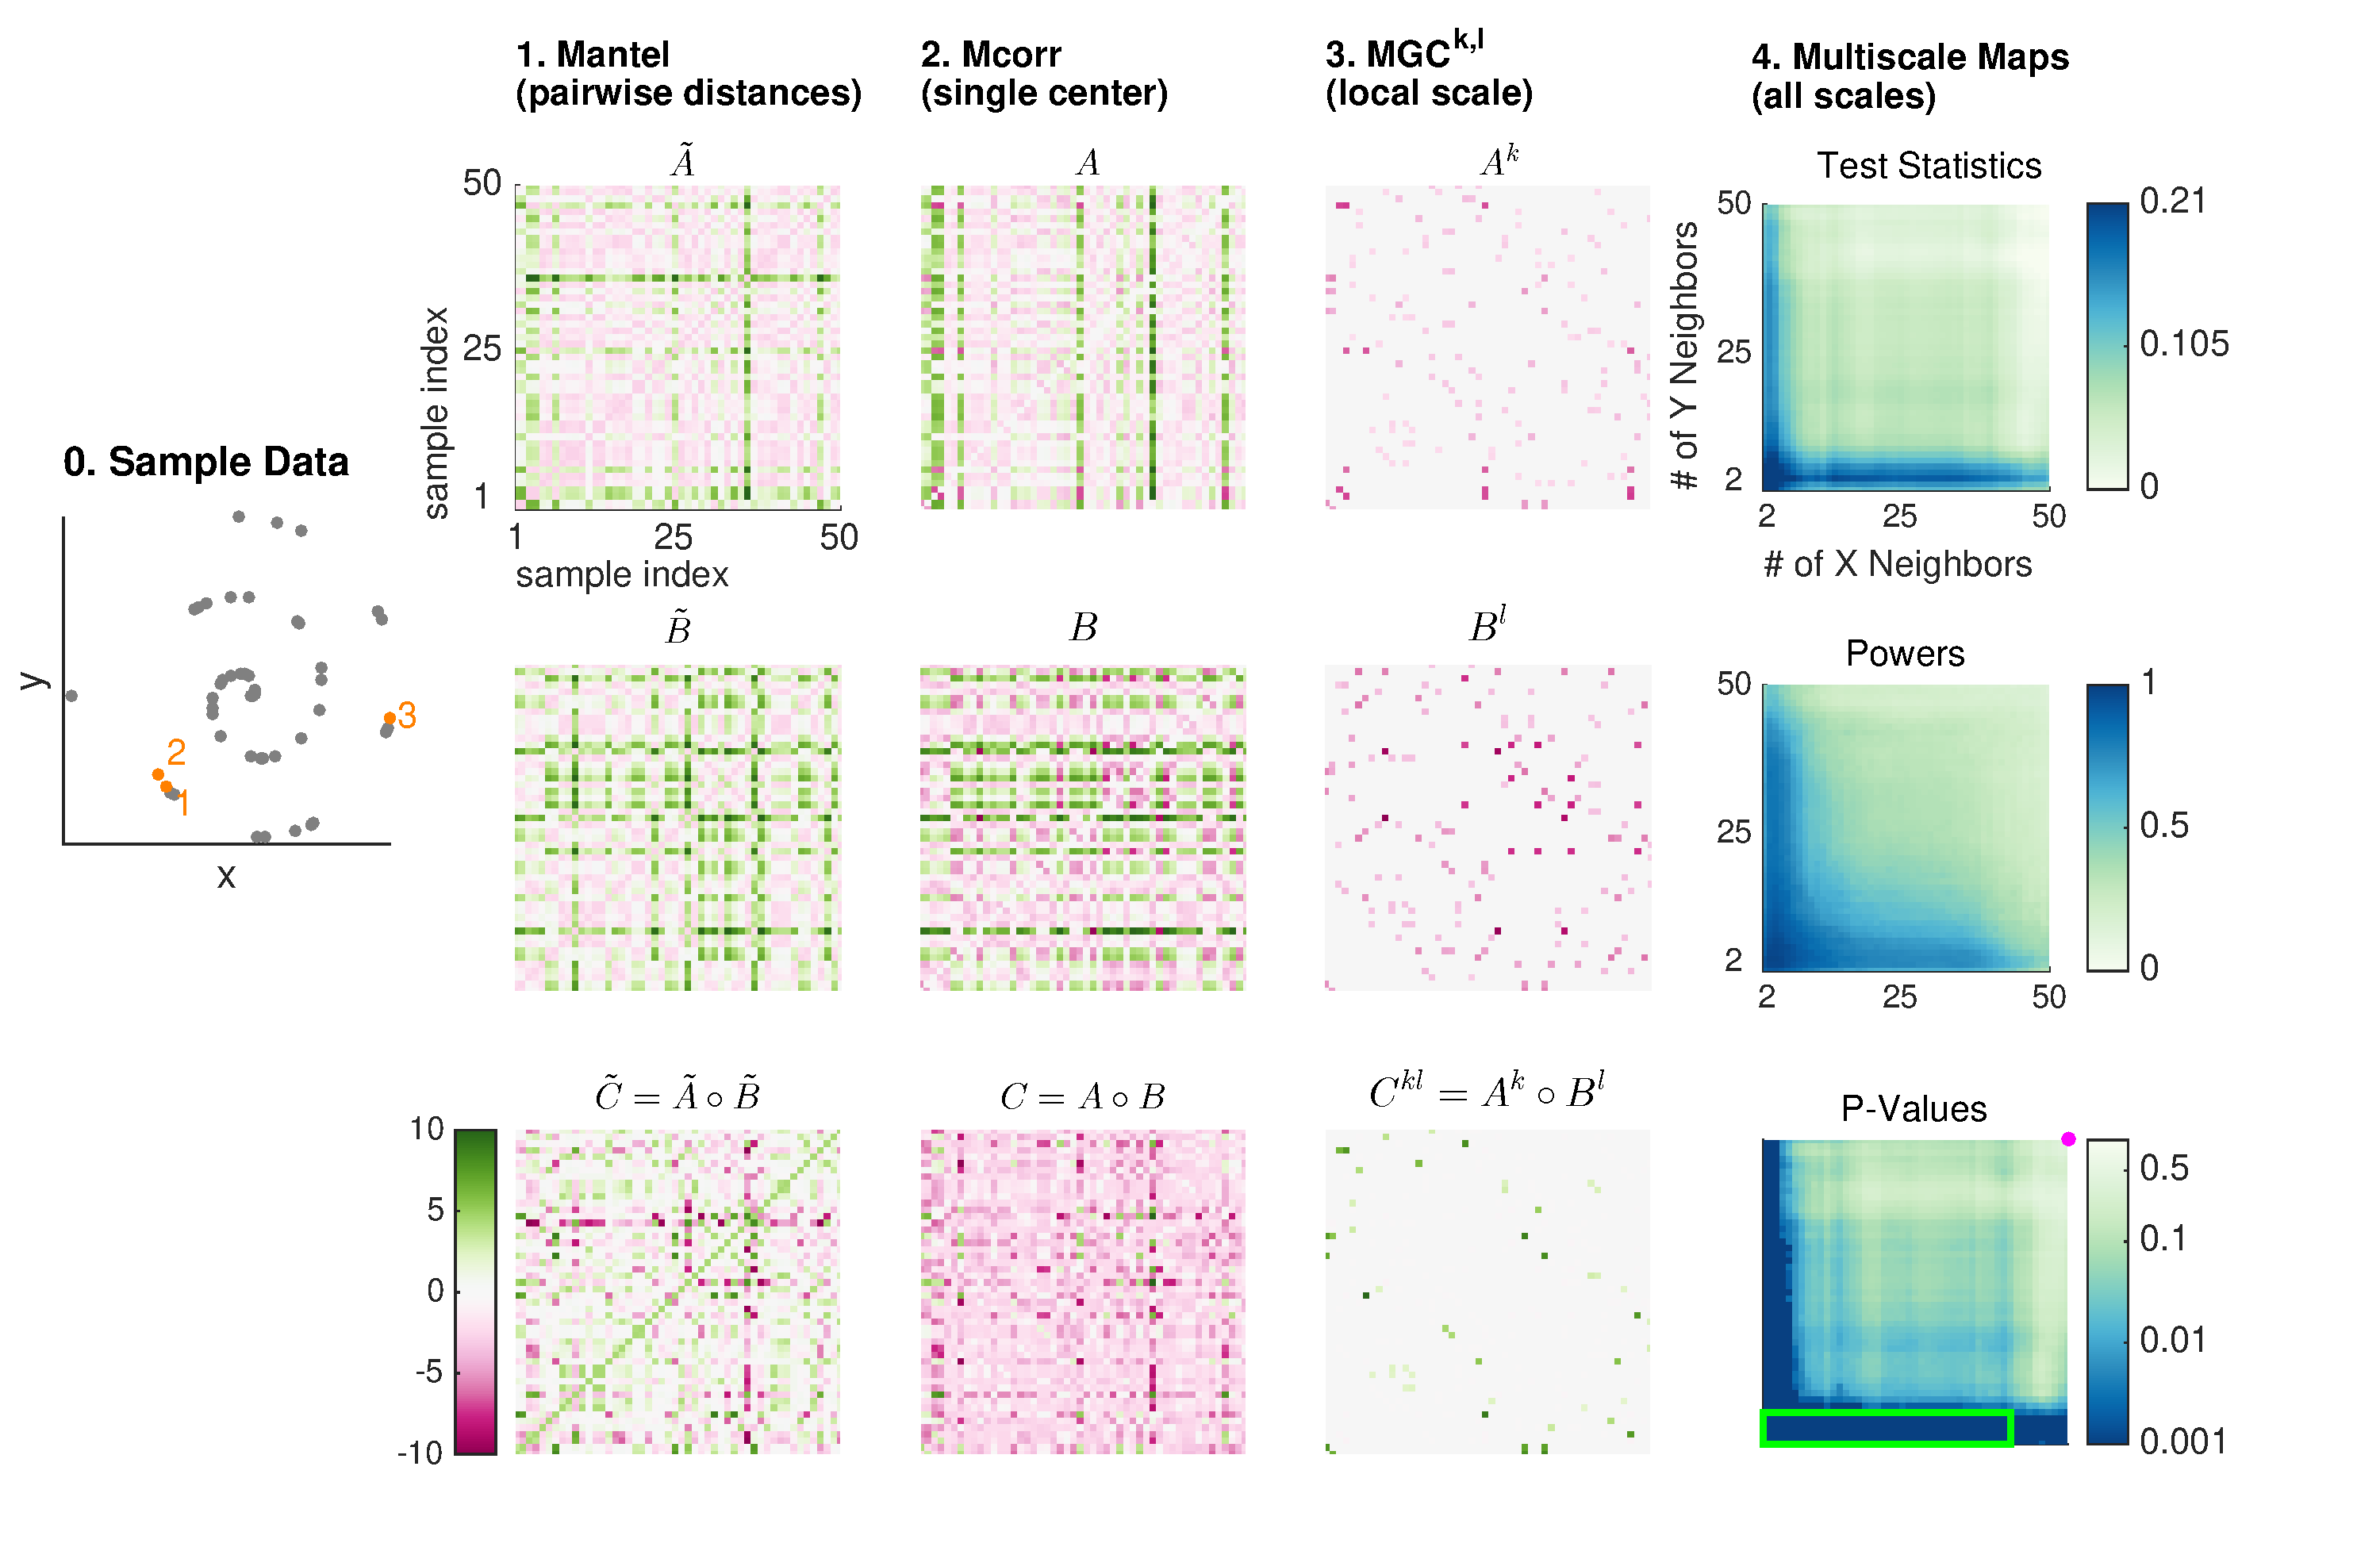
\includegraphics[width=1.0\textwidth]{../Figures/FigA}
\end{figure}
\end{frame}

\begin{frame}{Advantage of Utilizing Locality}
% \vspace{-35pt}\hspace{-150pt}
\begin{tabular}{c  c  c  c}
 & Mantel & Mcorr & MGC \\
 $\delta_x$(1,2) & \hspace{1.8em} \color{magenta}-2.42 \hspace{1.8em}  & \hspace{1.8em} \color{magenta}-5.21 \hspace{1.8em} & \hspace{1.8em} \color{magenta}-5.07 \hspace{1.8em}  \\ 
 $\delta_y$(1,2) & \color{magenta}-1.58 & \color{magenta}-0.91 & \color{magenta}-0.12  \\ 
 $\delta_x \times \delta_y$ & \color{blue}3.82 & \color{blue}4.74 & \color{blue}0.61  \\ 
 
\hline


 $\delta_x$(2,3) & \color{blue}0.70 & \color{blue}0.61 & \color{blue}0.14  \\ 
 $\delta_y$(2,3) &  \color{magenta}-0.91 & \color{magenta}-0.28 & \color{blue}0.12  \\ 
 $\delta_x \times \delta_y$ & \color{magenta}-0.63 & \color{magenta}-0.17 & \color{blue}0.02  \\ 

\hline
 $\sum{\delta_x \times \delta_y}$ & \color{magenta}-162.14   & \color{magenta}-93.04 & \color{blue}116.41  \\ 
$\sum{\delta_x \times \delta_y} / \sum{\delta_{x}^2}\sum{\delta_{y}^2}$ &  \color{magenta}-0.02  & \color{magenta}-0.02 & \color{blue}0.16  \\ 

\end{tabular}
\end{frame}

\subsection{Numerical Simulations}
\begin{frame}{Simulation Set-Up}
In total $20$ different joint distributions $f_{xy}$ are considered, including linear and nearly linear  (1-5), polynomial   (6-12), trigonometric (13-17), uncorrelated but nonlinearly dependent  (18-19), and an independent relationship (20).

\pause
\medskip
For each distribution, we further consider two different scenarios: a $1$-dimensional scenario with increasing sample size, and a high-dimensional scenario with fixed sample size and increasing dimensions (not shown in slides).

\pause
\medskip
The benchmarks are distance correlation, modified distance correlation, the Mantel test, and the HHG method proposed in [\textit{Heller et al.(2013)}]\cite{HellerGorfine2013}.

\pause
\medskip
Our \Mgc~implementation is based on modified distance correlation with single centering.
\end{frame}

\begin{frame}{Visualizations of Simulation Settings}
\begin{figure}[ht]
  \centering
  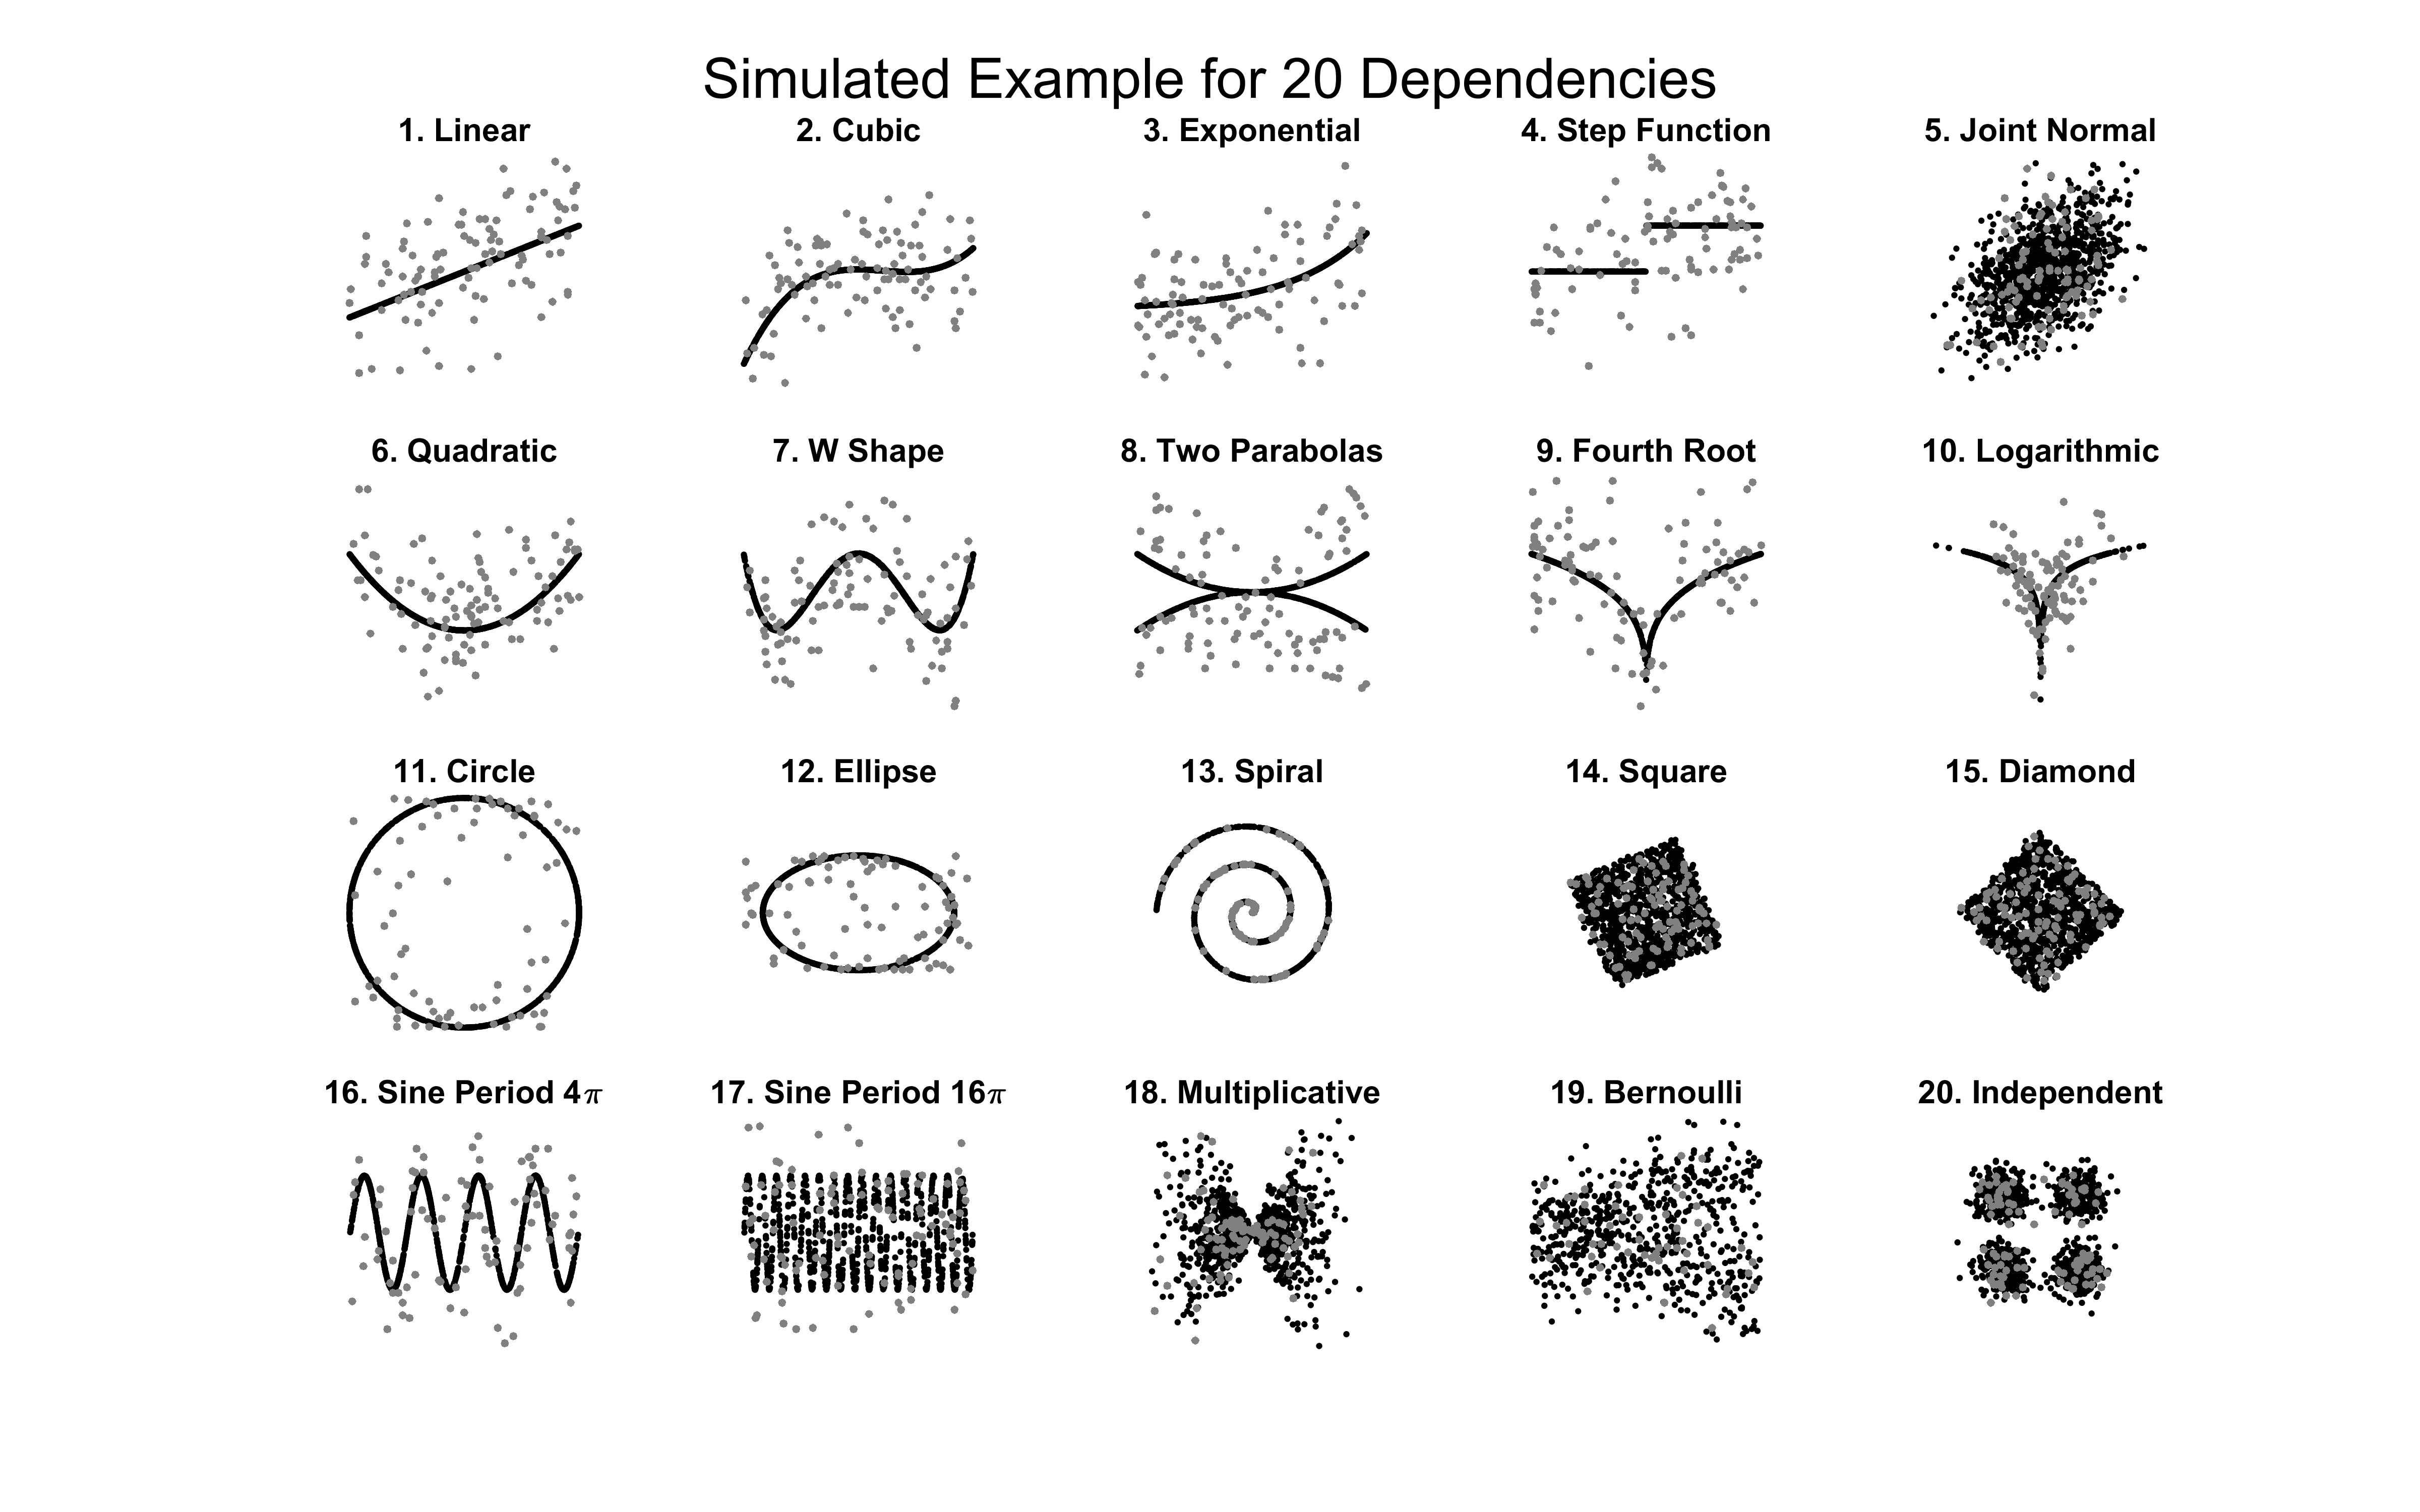
\includegraphics[width=0.9\textwidth]{../Figures/FigSimVisual}
	\caption{Visualization of the $20$ dependencies for one-dimensional simulations. 
}
	\label{f:dependencies}
\end{figure}
\end{frame}

\begin{frame}{Simulation Powers}
\begin{figure}[htbp]
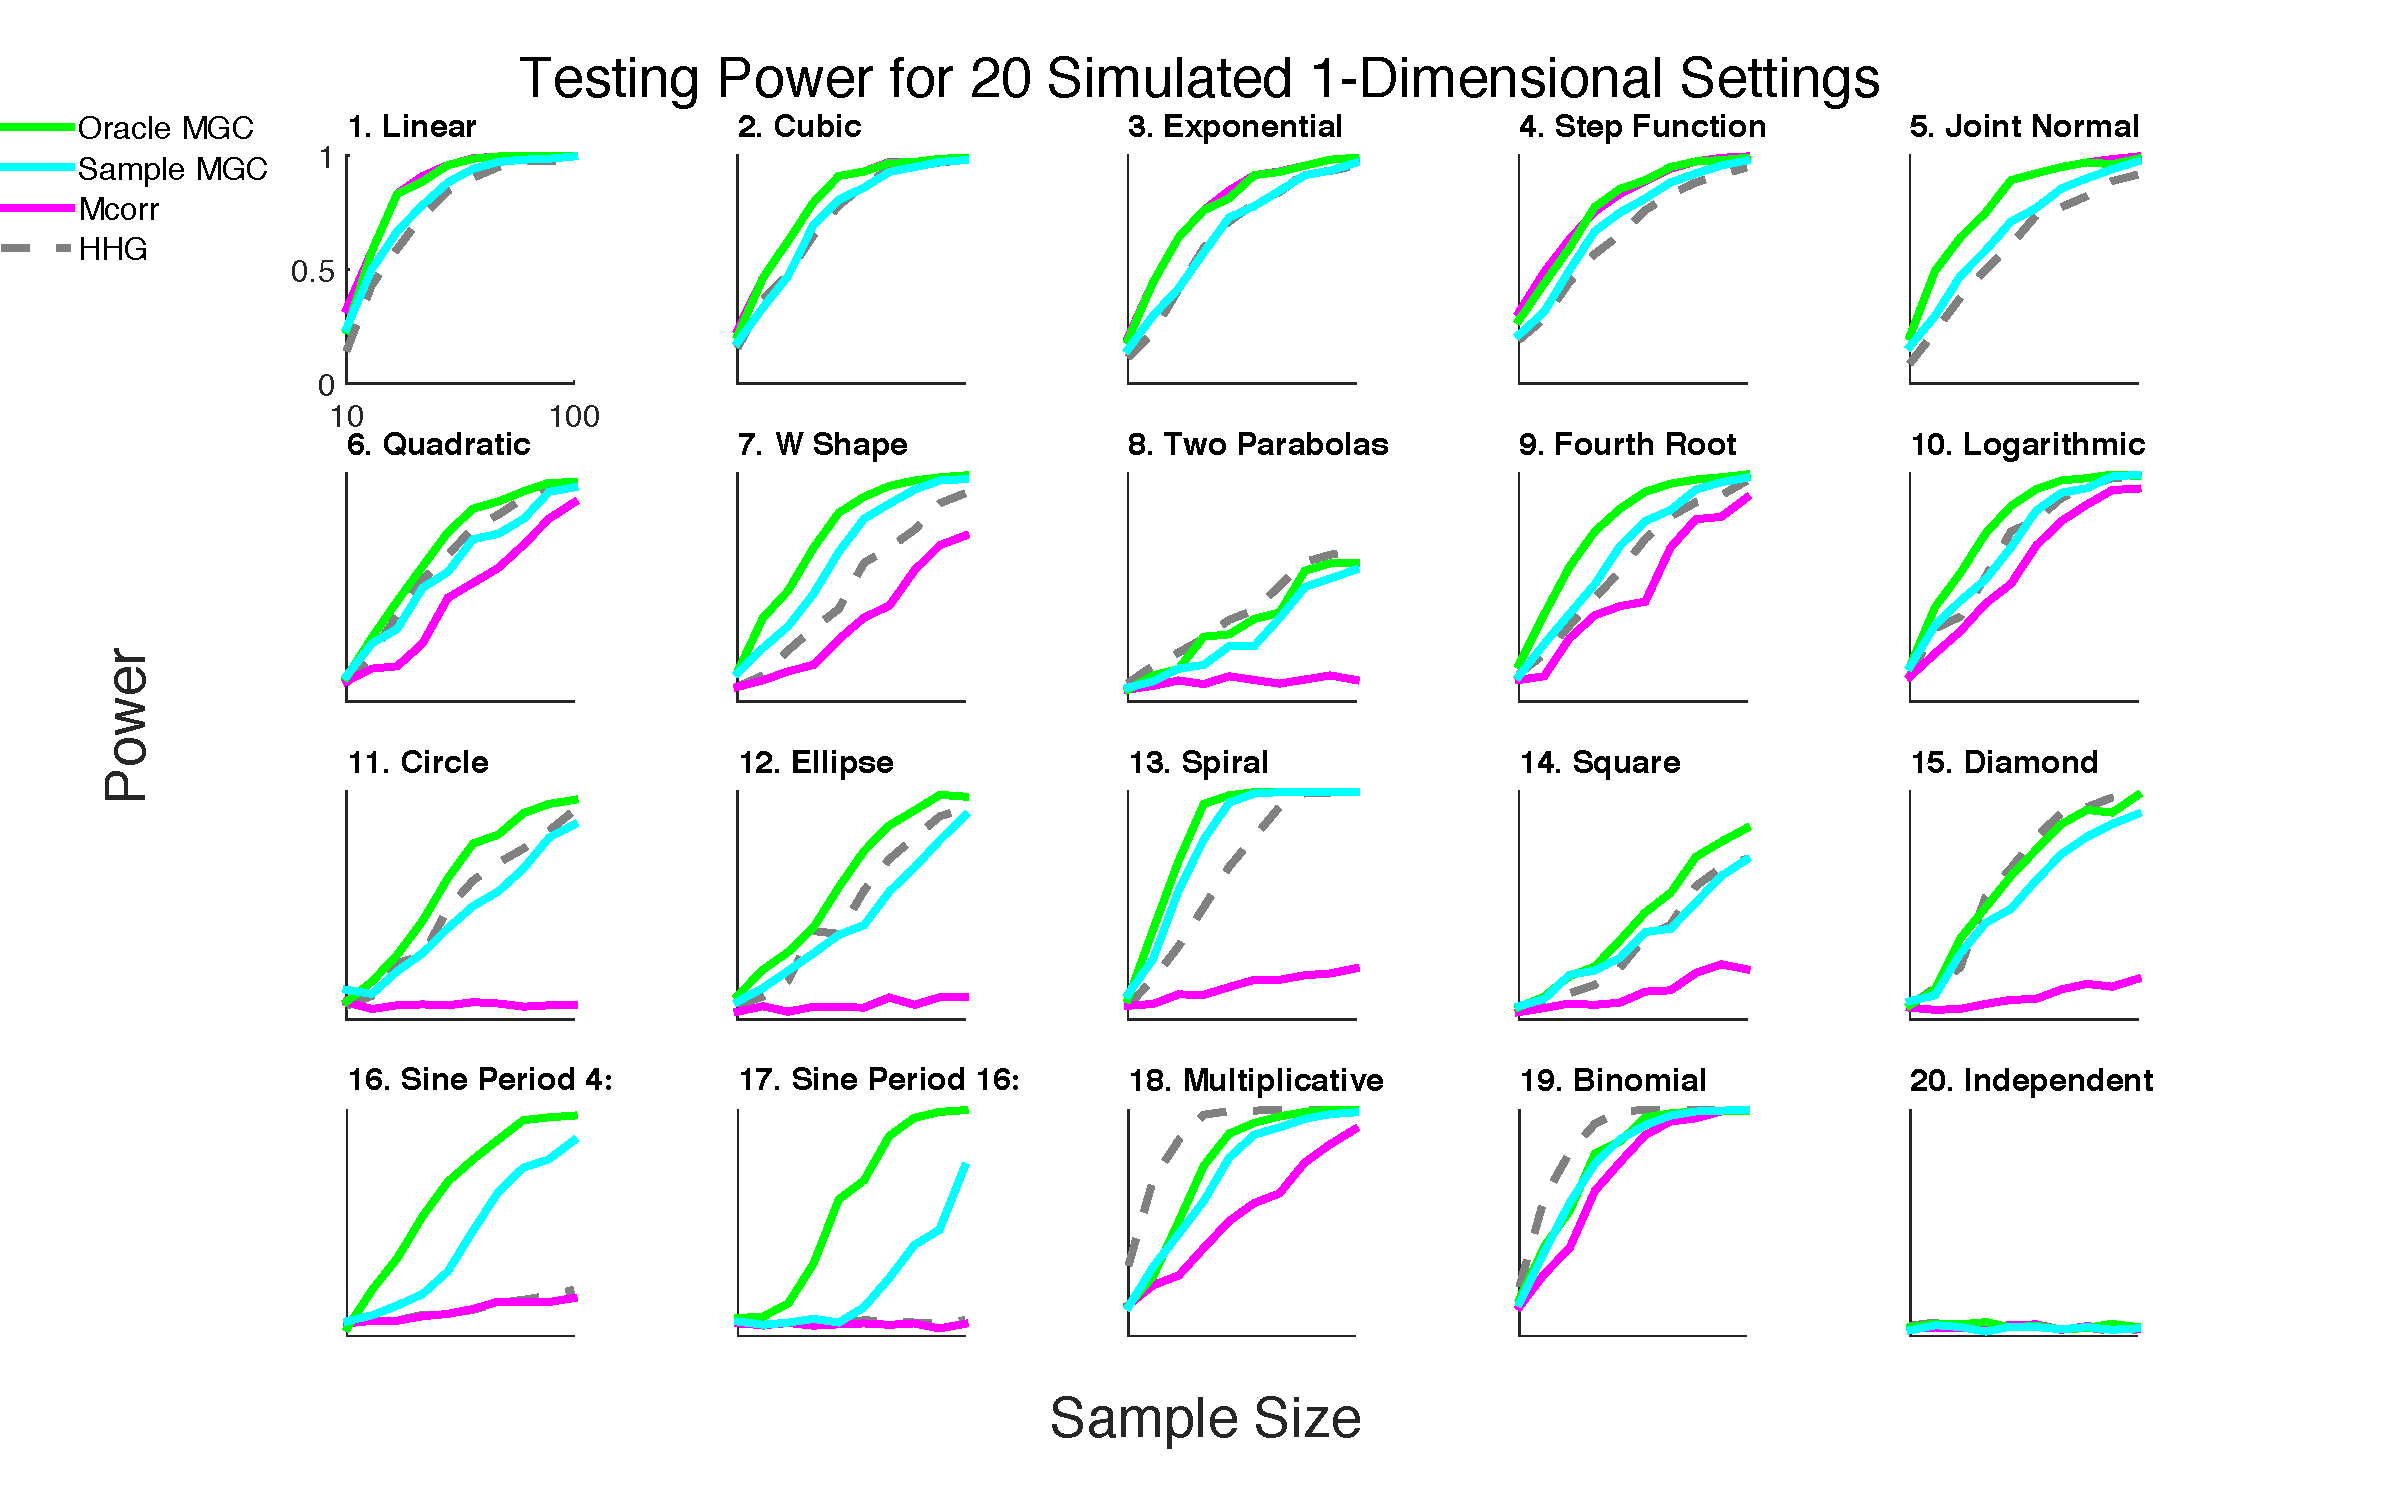
\includegraphics[width=0.9\textwidth]{../Figures/Fig1DPower}
\caption{
Powers of different methods for $20$ different one-dimensional dependence structures.}
\end{figure}
\end{frame}

\begin{frame}{Simulation Power Map}
\begin{figure}[htbp]
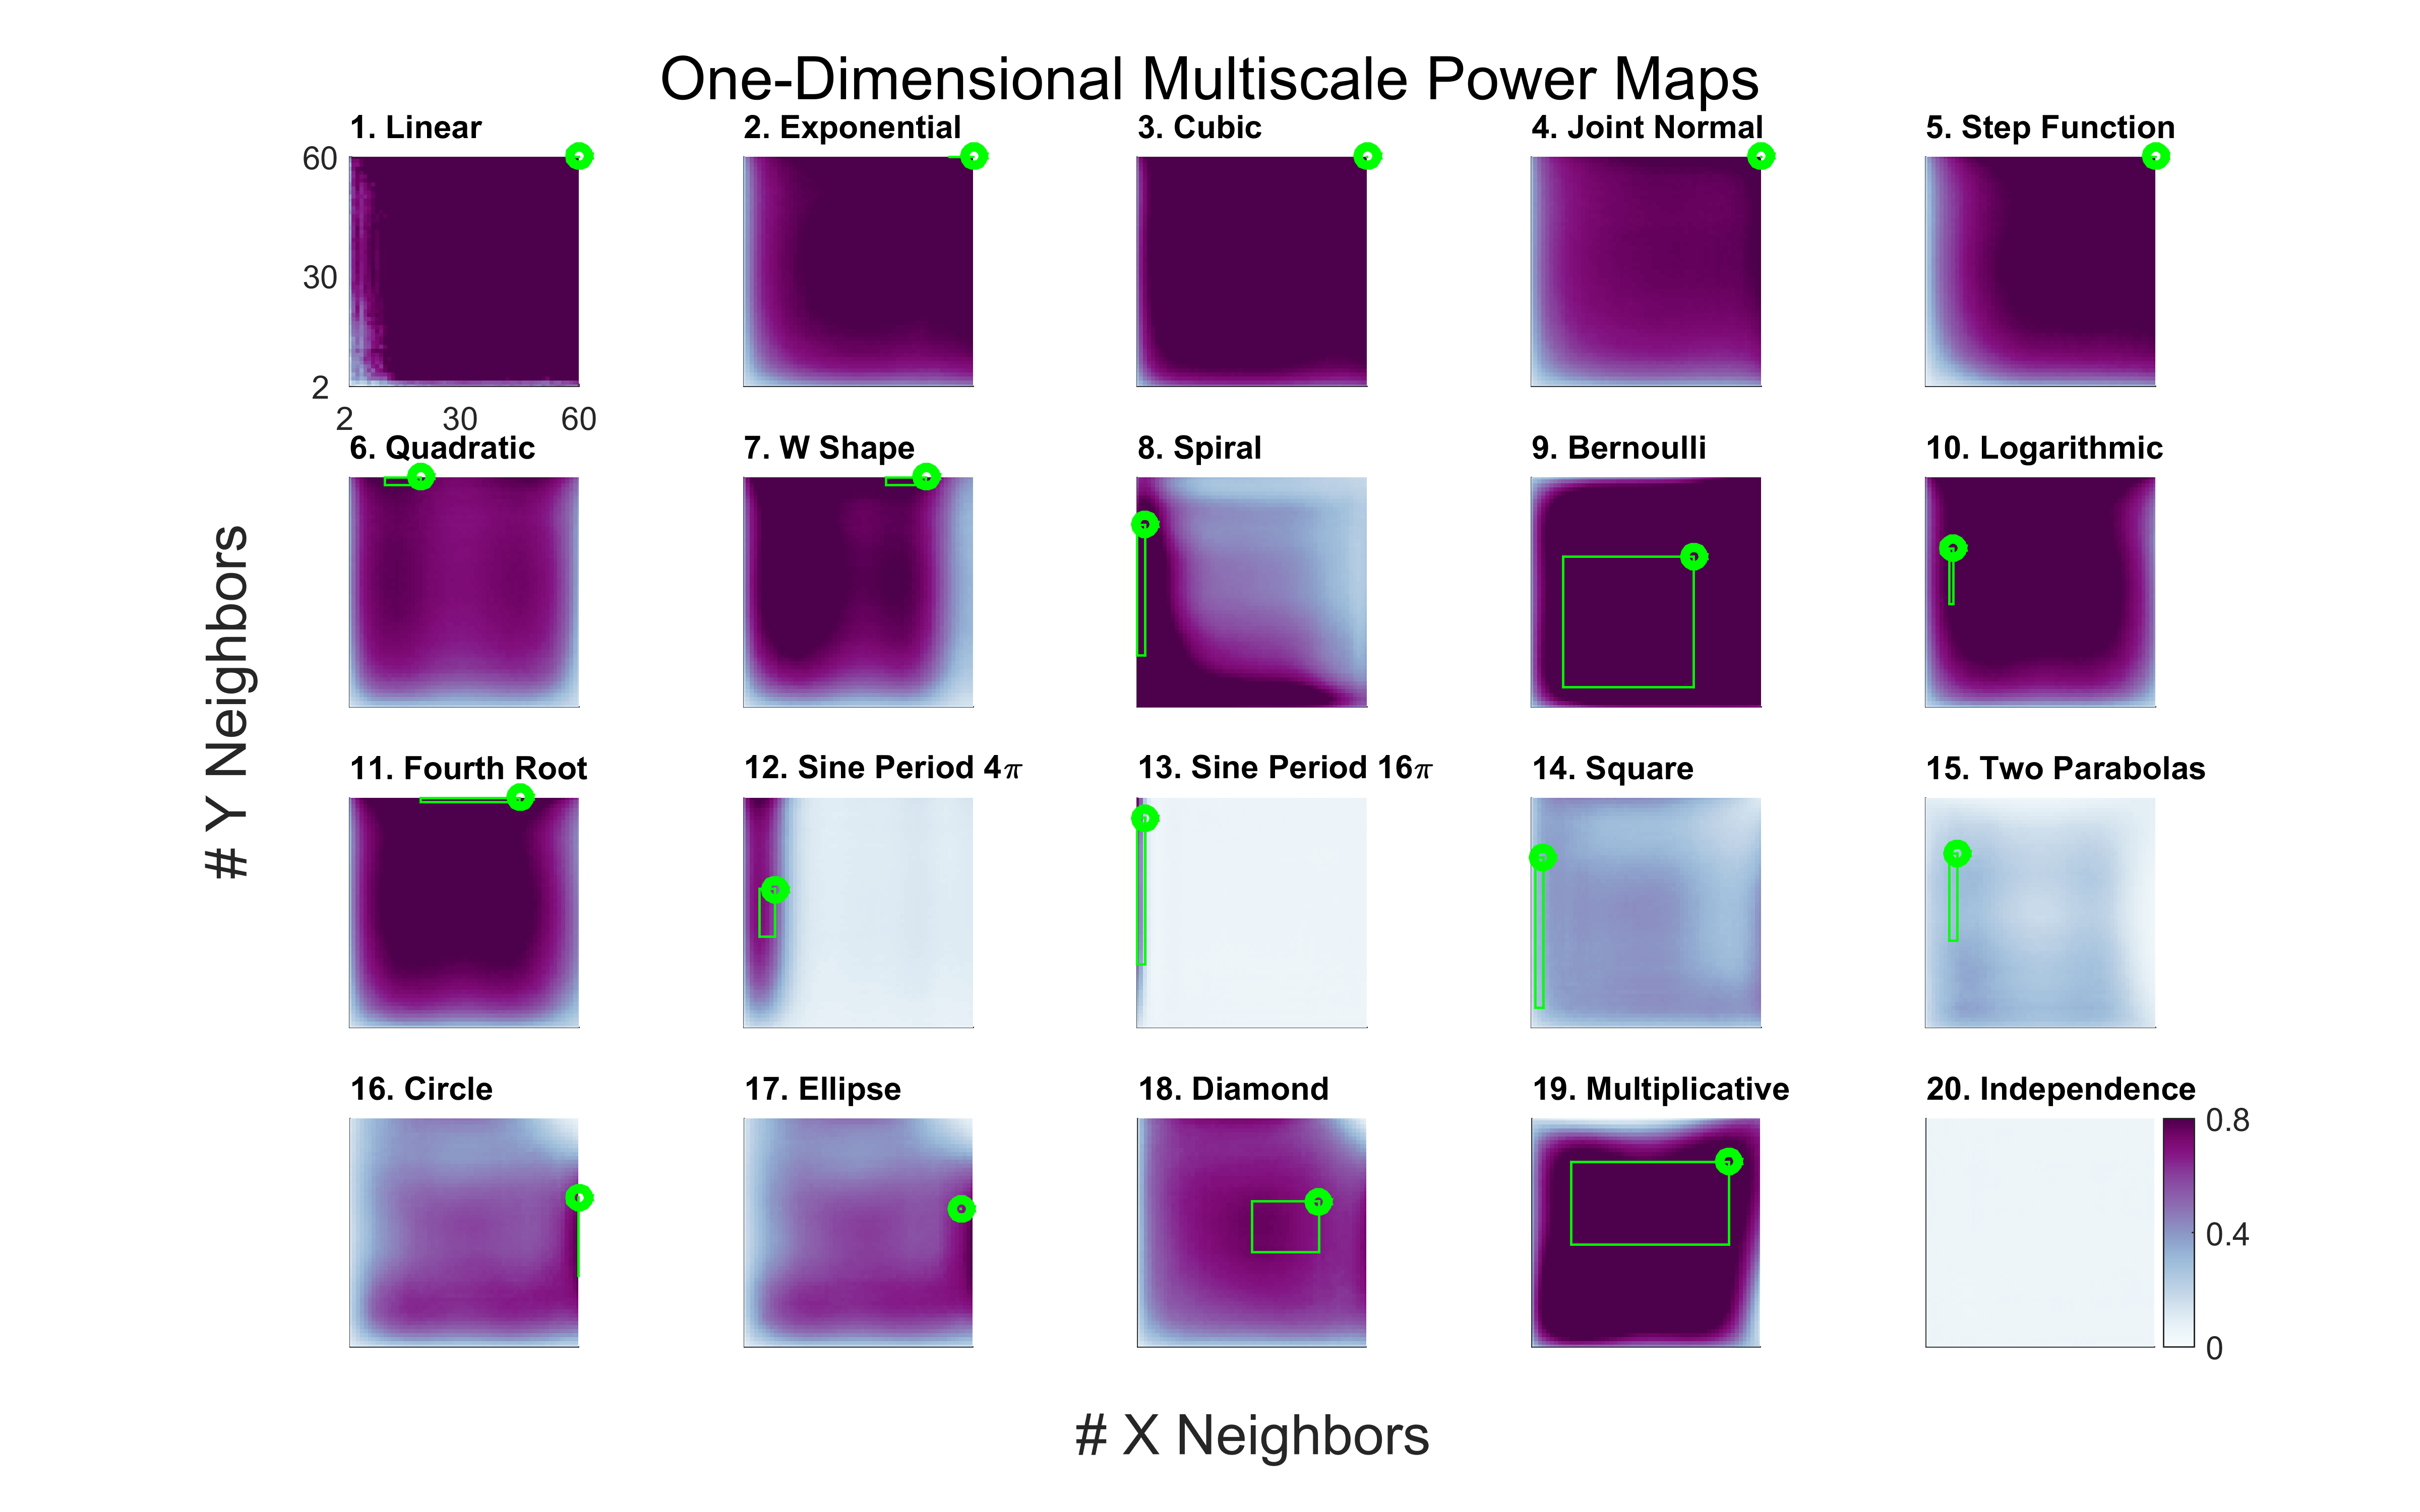
\includegraphics[width=0.9\textwidth]{../Figures/Fig1DHeat}
\caption{
Multiscale Power Maps indicating the influence of neighborhood size on \Mgc~testing power.}
\end{figure}
\end{frame}

\subsection{Real Data Experiments}
\begin{frame}{Brain vs Personality}
[\textit{Adelstein et al.(2011)}] \cite{AdelsteinEtAl2011} was able to detect dependence between certain brain regions and personality, but lacked the tools to test for dependence of the whole brain activity against all five dimensions of personality. 

\pause
\medskip 
In this dataset, we have $n=42$ subjects, for each we obtained  $197$ time-steps of resting-state functional MRI activity, as well as the five-factor personality trait as quantified by  the NEO Personality Inventory-Revised. 

\pause
\medskip 
The raw brain activity was processed using CPAC [\textit{Craddock et al.(2015)}]\cite{CPAC2015}. Then we ran a spectral analysis on each region, bandpassed and normalized it, and then calculated the Kullback-Leibler divergence across regions and the normalized Hellinger distance between each subject.  

\pause
\medskip 
For the five-factor personality data, we directly use the Euclidean distance.
\end{frame}

\begin{frame}{Permutation Test P-value map}
\begin{figure}[htbp]
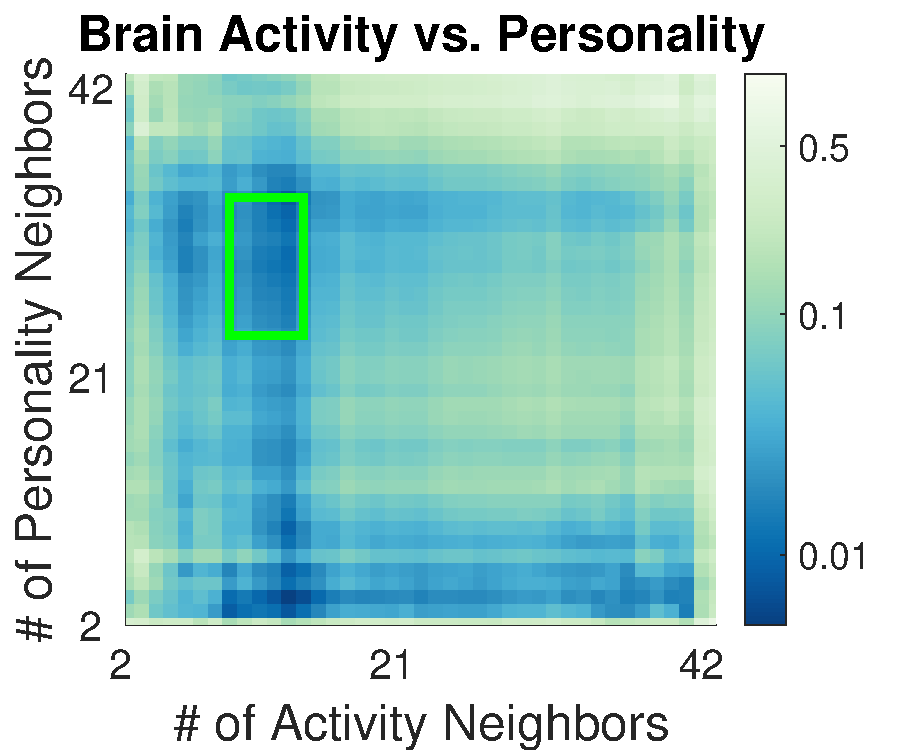
\includegraphics[width=0.7\textwidth]{../Figures/FigReal1}
\caption{P-value map (log scale) for brain fMRI scan vs five-factor personality.}
\label{f:realA}
\end{figure}
\end{frame}

\section{Conclusion}
\begin{frame}{Advantages of MGC}
\begin{itemize}[<+->]
\item 1) \Mgc~is consistent against all distributions of finite second moment when based on dcorr or mcorr.
\item 2) \Mgc~exhibits superior numerical performance in a comprehensive simulation setting, throughout various linear / nonlinear / high-dimensional / noisy dependencies.
\item 3) \Mgc~is easy and efficient to implement for any generalized correlation.
\item 4) \Mgc~not only outputs a p-value in testing, but also provides useful information on the local scale where the dependency is the strongest, and implies the geometry of the underlying dependency.
\end{itemize}
\end{frame}

\begin{frame}{What we do not show in slides}
\begin{itemize}[<+->]
\item \Mgc~superiority for high-dimensional simulations.
\item \Mgc~applications for brain shape vs disease, and brain activity vs fake movie.
\item \Mgc~implementation by single centered dcorr, which is equivalent to the original dcorr in testing but better preserves the rank information.
\item \Mgc~scale selection algorithm based on the p-value map, which heuristically selects the optimal scale by finding consecutive regions of significant p-values.
\end{itemize}
\pause
\medskip
And many other details...
\end{frame}

%\begin{frame}{What We Do Not Show In Slides}
%\begin{itemize}[<+->]
%\item MGC is robust against outliers;
%\item In case of one pair of given data of unknown model, how to choose the optimal scale heuristically;
%\item Real data experiments where MGC is used to detect local signals between brain data vs phenotypes.
%\end{itemize}
%\end{frame}

%\begin{frame}{In The Future}
%\begin{itemize}[<+->]
%\item Testing dependence on networks.
%\item Better optimal scale estimation for unknown model.
%\item Investigate alternative form of local correlations.
%\item Local correlation is potentially useful for nonlinear embedding, variable selection, etc.
%\end{itemize}
%\end{frame}

%tba: add PIE and WIKI GF data
%\begin{frame}[allowframebreaks]
%\frametitle{References}
%\tiny
%\bibliographystyle{ieeetr}
%\bibliography{references}

%\end{frame}
\begin{frame}[allowframebreaks]

%\frametitle{References}
\tiny
%\bibliographystyle{ieeetr}
\bibliography{MGCbib}

\end{frame}

%------------------------------------------------

%----------------------------------------------------------------------------------------

\end{document} 
